% Modified based on Xiaoming Sun's template
\documentclass{article}
\usepackage{amsmath,amsfonts,amsthm,amssymb}
\usepackage{setspace}
\usepackage{fancyhdr}
\usepackage{lastpage}
\usepackage{extramarks}
\usepackage{chngpage}
\usepackage{soul,color}
\usepackage{graphicx,float,wrapfig}
\usepackage{enumitem}
\usepackage{array} 
\newcommand{\Class}{Pattern Recognition and Machine Learning}

% Homework Specific Information. Change it to your own
\newcommand{\Title}{Homework 3}

% In case you need to adjust margins:
\topmargin=-0.45in      %
\evensidemargin=0in     %
\oddsidemargin=0in      %
\textwidth=6.5in        %
\textheight=9.0in       %
\headsep=0.25in         %

% Setup the header and footer
\pagestyle{fancy}                                                       %
\chead{\Title}  %
\rhead{\firstxmark}                                                     %
\lfoot{\lastxmark}                                                      %
\cfoot{}                                                                %
\rfoot{Page\ \thepage\ of\ \protect\pageref{LastPage}}                          %
\renewcommand\headrulewidth{0.4pt}                                      %
\renewcommand\footrulewidth{0.4pt}                                      %

%%%%%%%%%%%%%%%%%%%%%%%%%%%%%%%%%%%%%%%%%%%%%%%%%%%%%%%%%%%%%
% Some tools
\newcommand{\enterProblemHeader}[1]{\nobreak\extramarks{#1}{#1 continued on next page\ldots}\nobreak%
                                    \nobreak\extramarks{#1 (continued)}{#1 continued on next page\ldots}\nobreak}%
\newcommand{\exitProblemHeader}[1]{\nobreak\extramarks{#1 (continued)}{#1 continued on next page\ldots}\nobreak%
                                   \nobreak\extramarks{#1}{}\nobreak}%

\newcommand{\homeworkProblemName}{}%
\newcounter{homeworkProblemCounter}%
\newenvironment{homeworkProblem}[1][Problem \arabic{homeworkProblemCounter}]%
  {\stepcounter{homeworkProblemCounter}%
   \renewcommand{\homeworkProblemName}{#1}%
   \section*{\homeworkProblemName}%
   \enterProblemHeader{\homeworkProblemName}}%
  {\exitProblemHeader{\homeworkProblemName}}%

\newcommand{\homeworkSectionName}{}%
\newlength{\homeworkSectionLabelLength}{}%
\newenvironment{homeworkSection}[1]%
  {% We put this space here to make sure we're not connected to the above.

   \renewcommand{\homeworkSectionName}{#1}%
   \settowidth{\homeworkSectionLabelLength}{\homeworkSectionName}%
   \addtolength{\homeworkSectionLabelLength}{0.25in}%
   \changetext{}{-\homeworkSectionLabelLength}{}{}{}%
   \subsection*{\homeworkSectionName}%
   \enterProblemHeader{\homeworkProblemName\ [\homeworkSectionName]}}%
  {\enterProblemHeader{\homeworkProblemName}%

   % We put the blank space above in order to make sure this margin
   % change doesn't happen too soon.
   \changetext{}{+\homeworkSectionLabelLength}{}{}{}}%

\newcommand{\Answer}{\ \\\textbf{Answer:} }
\newcommand{\Acknowledgement}[1]{\ \\{\bf Acknowledgement:} #1}

%%%%%%%%%%%%%%%%%%%%%%%%%%%%%%%%%%%%%%%%%%%%%%%%%%%%%%%%%%%%%


%%%%%%%%%%%%%%%%%%%%%%%%%%%%%%%%%%%%%%%%%%%%%%%%%%%%%%%%%%%%%
% Make title
\title{\textmd{\bf \Class: \Title}}
  \date{\textbf{\today}}
\author{\textbf{Qingru Hu \quad 2020012996}}
%%%%%%%%%%%%%%%%%%%%%%%%%%%%%%%%%%%%%%%%%%%%%%%%%%%%%%%%%%%%%

\begin{document}
\begin{spacing}{1.1}
\maketitle \thispagestyle{empty}

%%%%%%%%%%%%%%%%%%%%%%%%%%%%%%%%%%%%%%%%%%%%%%%%%%%%%%%%%%%%%
% Begin edit from here

\begin{homeworkProblem}
% \Answer \\
The loss function for LDA (using Fisher's condition) is:
\begin{equation}
  l_{\text{LDA}} = \frac{1}{2} (\boldsymbol{w}^{\top} \boldsymbol{x}_i + b - y_i)^2
\end{equation}
The loss function for logistic regression is:
$$
l_{\text{LG}}(x)=\left\{
\begin{aligned}
-\log(\theta(x)) \quad y_i = 1\\
-\log(1-\theta(x)) \quad y_i = 0
\end{aligned}
\right.
$$
where $\theta(x) = \frac{e^{\boldsymbol{w}^{\top} \boldsymbol{x}_i + b}}{1 + e^{\boldsymbol{w}^{\top} \boldsymbol{x}_i + b}}$
\end{homeworkProblem}.
The loss function of soft SVM is:
\begin{equation}
  l_{\text{hinge}}(x) = \max(1 - y_i\cdot (\boldsymbol{w}^{\top} \boldsymbol{x}_i + b), 0)
\end{equation}

For a concrete class $y=1$, plot curves of the three loss functions in Fig.\ref{loss_func}.
\begin{figure}[H]
  \begin{center}
    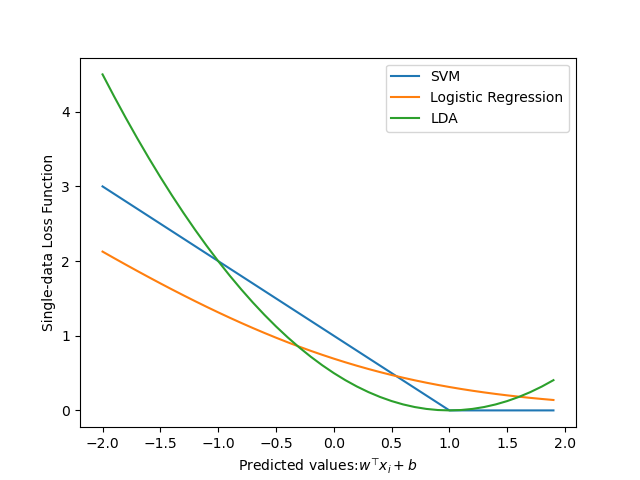
\includegraphics[width=8cm]{loss_func.png}
  \end{center}
  \caption{The single-data loss function for the three methods}
  \label{loss_func}
\end{figure}

In LDA, every sample in the dataset contributes to the loss function if it is wrongly classified, so 
LDA is somewhat prone to outliers.

In Logistic Regression, we punish those totally misclassified points severely, but don't pay much attention to those 
data that are most difficult to classify, so it is robust to outliers but may misclassify those ambiguous ones.

In SVM, only those points that are most difficult to discriminate (near the hyperplane) contibute to the total loss function, 
so it may be able to classify those samples near the hyperplane well and is prone to outliers.


\begin{homeworkProblem}
  The \textbf{hard-margin} problem is:
  \begin{align*}
    & \mathop{\text{min}}\limits_{\boldsymbol{w}, b} \frac{1}{2}\Vert \boldsymbol{w} \Vert ^2 \\
    \text{s.t.} & \quad y_i \cdot (\boldsymbol{w}^{\top}\boldsymbol{x}_i+b) \geq 1,\ 0 \leq i \leq n.
  \end{align*}
The Lagrangian function is:
\begin{align*}
L(\boldsymbol{w}, b, \alpha, \xi, \mu) & = 
\frac{1}{2} \Vert \boldsymbol{w} \Vert_{2}^2 + \sum_{i=1}^n\alpha_i [1 - y_i (\boldsymbol{w}^{\top}x_i + b)] \\
& \alpha_i \geq 0, i=1, \dots, n
\end{align*}
Take the partial derivatives of Lagrangian w.r.t $\boldsymbol{w}$,$b$ 
and set to zero:
\begin{align*}
  \frac{\partial L}{\partial \boldsymbol{w}}  = 0 \quad \boldsymbol{w} = \sum_{i=1}^{n} \alpha_iy_ix_i\\
\frac{\partial L}{\partial b} = 0 \quad \sum_{i=1}^{n} \alpha_iy_i = 0\\
\end{align*}
Pluge the above relations into the original Lagrangian function 
and we can get:
\begin{align*}
  L(\boldsymbol{w}, b, \alpha, \xi, \mu) &= 
  \frac{1}{2} \boldsymbol{w}^{\top} \boldsymbol{w} + 
  \sum_{i=1}^{n} \alpha_i - \sum_{i=1}^{n} \alpha_i y_i (\boldsymbol{w}^{\top}x_i + b) \\
  &= \frac{1}{2} (\sum_{i=1}^{n} \alpha_iy_ix_i)^{\top}(\sum_{i=1}^{n} \alpha_iy_ix_i)
   + \sum_{i=1}^{n} \alpha_i - \sum_{i=1}^{n} (\alpha_i y_i (\sum_{j=1}^{n} \alpha_j y_j x_j)^{\top}x_i) \\
  &= \sum_{i=1}^{n}\alpha_i - \frac{1}{2}\sum_{i=1}^{n}\sum_{j=1}^n \alpha_i \alpha_j y_i y_j \boldsymbol{x}_i^{\top} \boldsymbol{x}_j \\
  %\text{s.t.}\sum_{i=1}^{n}\alpha_iy_i = 0, 0\leq \alpha_i \leq C, i=1, \dots, n
  \end{align*}
Therefore, the original optimal problem is equivalent to the dual problem:
\begin{align*}
  \mathop{\text{max}}\limits_{\alpha} \sum_{i=1}^{n}\alpha_i - \frac{1}{2}\sum_{i=1}^{n}\sum_{j=1}^n \alpha_i \alpha_j y_i y_j \boldsymbol{x}_i^{\top} \boldsymbol{x}_j \\
  \text{s.t.}\sum_{i=1}^{n}\alpha_iy_i = 0, \alpha_i \geq 0, i=1, \dots, n
\end{align*}
Denote the solution in the first problem as $\boldsymbol{w}^*$ and solution in the second problem as $\boldsymbol{\alpha}^*$, 
and the solutions satisfy:
\begin{align*}
  \boldsymbol{w}^* = \sum_{i=1}^{n} \alpha_i^* y_ix_i
\end{align*}
From the complementary slackness of KKT conditions, we have:
\begin{align*}
  \alpha_i [1 - y_i (\boldsymbol{w}^{\top}x_i + b)] = 0
\end{align*}
If $\alpha_i>0$, then $y_i (\boldsymbol{w}^{\top}x_i + b) = 1$.
Notice that $y_i = \pm 1$, so $\boldsymbol{w}^{\top}x_i + b = y_i$.

\end{homeworkProblem}

\begin{homeworkProblem}
  Search the paper and conduct a literature review for how to add different regularizations to SVM, 
  and more sophisticated forms of kernel function.

\Answer
Classical
regularization theory formulates the regression and classification problem as
a variational problem of finding the function f that minimizes the functional:
\begin{equation}
  \mathop{\text{min}}\limits_{f \in H} H[f] = \frac{1}{l}\sum_{i=1}^{l} V(y_i, f(\boldsymbol{x}_i))
   + \lambda \Vert f \Vert^2_{K}
\end{equation}
where $\Vert f \Vert^2_{K}$ is a norm in a Reproducing Kernel Hilbert Space $H$ 
defined by the positive definite function $K$, $l$ is the number of data points 
, $\lambda$ is the regularization parameter and $V(\cdot)$ is the loss function. Under rather general conditions 
the solution of the above equation is:
\begin{equation}
  f(\boldsymbol{x}) = \sum_{i=1}^{l} c_iK(\boldsymbol{x}, \boldsymbol{x}_i) + b
\end{equation}
For a classical ($L_2$) Regularization Networks (RN), the loss function is:
\begin{equation}
  V(y_i, f(\boldsymbol{x}_i)) = (y_i - f(\boldsymbol{x}_i))^2
\end{equation}
For Support Vector Machine Regression (SVMR), the loss function is:
\begin{equation}
  V(y_i, f(\boldsymbol{x}_i)) = \vert y_i - f(\boldsymbol{x}_i) \vert_{\epsilon}
\end{equation}
For Support Vector Machine Classification (SVMC), the loss function is:
\begin{equation}
  V(y_i, f(\boldsymbol{x}_i)) = \vert 1 - y_i f(\boldsymbol{x}_i) \vert_{+}
\end{equation}
where $|\cdot |_{\epsilon}$ is Vapnik's epsilon-insensitive norm, 
$|x|_+ = x$ if x is positive
and zero otherwise, and $y_i$ is a real number in RN and SVMR, whereas it takes values
-1, 1 in SVMC.

The different regularizations lie in the different norms $\Vert f \Vert^2_{K}$ 
in a Reproducing Kernel Hilbert Space $H$.


\end{homeworkProblem}

\begin{homeworkProblem}
\section*{(a) Use SVM to classify the train set and predict on the test set}
Use Linear SVM to classify the samples on the training set, and 
the accuracy on the test set is $97\%$.

\section*{(b) Different kernel functions and penalty strength $C$}
\begin{table}[htbp]
  \centering
  \begin{tabular}[htbp]{|c|c|c|}
    \hline
    Kernel & Penalty Strength & Accuracy(\%) \\
    \hline
    Linear & 0.1 & 96 \\
    \hline
    Poly & 0.1 & 79 \\
    \hline
    RBF & 0.1 & 84 \\
    \hline
    Sigmoid & 0.1 & 86 \\
    \hline 
    Linear & 1 & 96 \\
    \hline
    Poly & 1 & 83 \\
    \hline
    RBF & 1 & 97 \\
    \hline
    Sigmoid & 1 & 81 \\
    \hline 
    Linear & 10 & 96 \\
    \hline
    Poly & 10 & 90 \\
    \hline
    RBF & 10 & 97 \\
    \hline
    Sigmoid & 10 & 76 \\
    \hline 
  \end{tabular}
  \caption{Different kernel functions and penalty strength for SVM}
\end{table}
The best composition is the RBF kernel with a penalty strength 
of 1 or 10, which both have an accuracy of 97\%.

\section*{(c)  The supporting vectors}


\end{homeworkProblem}


% \newpage
% \Acknowledgement{Thank Siying Yang 2020012981 for
% the discussion about Problem 2.3 and Problem 3.}

% End edit to here
%%%%%%%%%%%%%%%%%%%%%%%%%%%%%%%%%%%%%%%%%%%%%%%%%%%%%%%%%%%%%

\end{spacing}
\end{document}

%%%%%%%%%%%%%%%%%%%%%%%%%%%%%%%%%%%%%%%%%%%%%%%%%%%%%%%%%%%%%
